\documentclass[11pt]{article}
\usepackage{fontspec,hyperref}
\usepackage[]{graphicx}
\DeclareGraphicsExtensions{.png}
\usepackage{listings}
\usepackage{color}
\usepackage[BoldFont,SlangFont,CJKchecksingle]{xeCJK}
%载入粗体,斜体,禁止单个汉字一行

%\setCJKmainfont{AR PL KaitiM GB}
\setCJKmainfont{AR PL SungtiL GB} %缺省汉字字体为简体
\setCJKfamilyfont{kai}{AR PL KaitiM GB}
\setCJKfamilyfont{hei}{WenQuanYi Zen Hei}

%\setmainfont{DejaVu Sans Mono:style=Book}
\XeTeXlinebreaklocale "zh"  %断行设置为中文格式
\XeTeXlinebreakskip=0pt plus 1pt minus 0.1pt

\title{文件读写模式}
\author{刘宇辉 \texttt{wolfpythonlondon@gmail.com}}
\date{\today}

\begin{document}
\maketitle

文件分为二进制文件和文本文件,文件的读写模式分为二进制模式和文本模式。文本
文件的表示基本上就是字符在计算机系统内部的表示。比如:\\
7896,在文本文件中,就是7,8,9,6对应的ansii码,而在二进制文件中,则是7896这个
数字的二进制表示,可以是0001111011011000,也可能是00000000000000000001111011011000,
具体的要看数据类型。\\

而二进制模式和文本模式本质上和二进制和文本文件没有关系。也就是说,以二进制
模式打开读写的文件不一定是二进制文件,同理以文本模式打开读写的文件也不一定
是文本文件。二进制模式指的是,内存缓冲区里面是什么,就输出什么,比如缓冲区里是2345,
那么输出的时候,就输出2345。文本模式在Windows上是,写操作时,对内存里的LF(\texttt{$\backslash$n}),进行替换
,替换为CR
LF两个字符,那么实际在磁盘上存储的文件就多了一个字符,读操作时,就是
就是逆过程。这个过程对于应用程序是看不到的,是Windows内核来做的。在Unix中,
文本模式和二进制模式没有什么区别,内核不会查看数据进行替换。\\

在Windows上的编辑器,比如notepad++,可以选择“显示所有字符”,这样就可以看到磁盘的文本文件里“原生态”的字符,
而不是被Windows内核处理过的文件。原理也就是
在打开文本文件的时候,选择二进制模式。\\

我使用跨平台的轻型IDE Geany来演示。


\lstset{language=C++,
        %backgroundcolor=\color{green},
        numbers=left,
        basicstyle=\ttfamily\small,
        keywordstyle=\color{red}\ttfamily,
        identifierstyle=\color{blue}\ttfamily,
        stringstyle=\ttfamily,
        commentstyle=\ttfamily,
        caption=\lstname,
        captionpos=b}

%\lstinputlisting[name=simplec.c]{../code/etip/simplec.c}
\begin{lstlisting}[name=test.cpp]
#include <iostream>
#include <fstream>

using namespace std;

int main()
{
	fstream out;
	fstream out1;
	int a = 7896;
	int b = 345;

	out.open("test",fstream::binary|fstream::out);
	out1.open("test1",fstream::out);

	out << a <<endl<<b;
	out1 << a <<endl<<b;
}
\end{lstlisting}

我们向文本文件test和test1里面分别用文本模式和二进制模式写入了两个数7896,345.
然后,分别用编辑器打开这两个文本文件,在显示时,选择显示行尾,这样我们
就能够看到在行末的字符(硬盘上存储的文件,而不是经过内核处理过存在于内存中的
文件)。\\

\begin{figure}
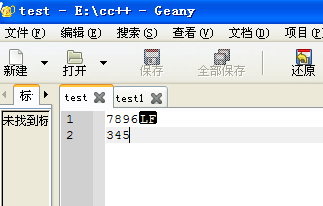
\includegraphics[scale=0.7]{/home/wolf/public/notes/blogs/img/Screenshot-2}
\caption{test(binary mode) in Windows}
\label{test(binary mode in windows}
\end{figure}
\begin{figure}
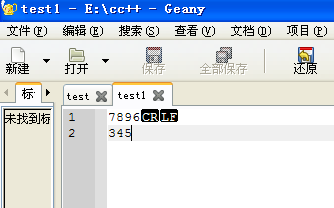
\includegraphics[scale=0.7]{/home/wolf/public/notes/blogs/img/Screenshot-3}
\caption{test1(text mode) in Windows}
\label{test1(text mode) in windows}
\end{figure}
\begin{figure}
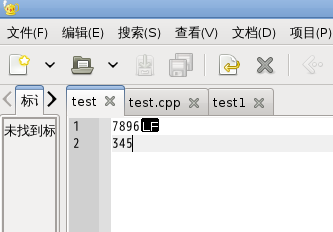
\includegraphics[scale=0.7]{/home/wolf/public/notes/blogs/img/Screenshot-4}
\caption{test(binary mode) in Debian}
\label{test(binary mode) in Debian}
\end{figure}
\begin{figure}
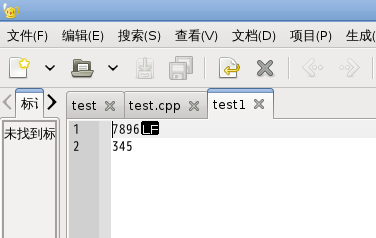
\includegraphics[scale=0.7]{/home/wolf/public/notes/blogs/img/Screenshot-5}
\caption{test1(text mode) in Debian}

\label{test1(text mode) in Debian}
\end{figure}

我们可以清楚的看到在实际硬盘存储中,Windows上经过text
mode写入的文件,在行末都会有一个CF字符,这个字符是不可见字符(那为什么我们又
看到了呢?这是一种表示方式而已:-)),而binary mode和Linux上的两种模式写入的文件
都没有多余的字符。我们再来看一下文件的大小,从而比较一下:
\begin{figure}
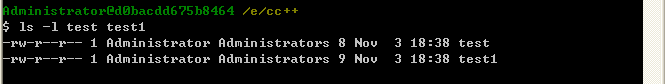
\includegraphics[scale=0.7]{/home/wolf/public/notes/blogs/img/Screenshot-6}
\caption{Windows上的文件大小}
\end{figure}
\begin{figure}
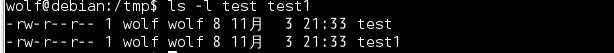
\includegraphics[scale=0.7]{/home/wolf/public/notes/blogs/img/Screenshot-7}
\caption{Debian上的文件大小}
\end{figure}
在实际的磁盘上,Windows上经text mode写入的文件test1,比经binary
mode写入的文件test
大了一个字节,这个字节就是CF字符。而Linux上则是相同的。










\end{document}
